\chapter{Planning the tracker calibration}
\textit{Reconstructing cosmic tracks and understanding resolutions require calibrating the tracker station. 
The primary goal of this calibration is to determine signal propagation and channel-to-channel 
delays for each straw. To achieve this, an unbiased reconstruction of the longitudinal position of the straw 
hit is essential. In this chapter, I will discuss the planning of the calibration using cosmic muons. My task 
involved reconstructing the cosmic trajectories in a vertically oriented station and understanding the potential 
biases and systematic errors that this orientation might introduce. }
\section{Overview of the timing calibration}
As mentioned in the introduction to this chapter, the main goal of this calibration is to determine signal propagation and channel-to-channel delays for each straw.
When a particle creates a signal in a straw, it propagates towards both ends. 
The arrival times at the ends will be called $t_1$ and $t_2$:
\begin{equation}
\begin{aligned}
    t_1 &= \frac{x_{\text{hit}}}{v} + t_0 + d_1 \\
    t_2 &= \frac{L - x_{\text{hit}}}{v} + t_0 + d_2
\end{aligned}
\end{equation}
where $L$ is the length of the straw, $x_{\text{hit}}$ is the straw hit position 
of the particle, $v$ is the propagation velocity inside the straw, $t_0$ the particle arrival time and $d_i$ 
are the delays introduced for the response of each end. $t_1$ and $t_2$ will be determined by the TDC timing on the HV side and on the CAL side.
The measurement of $\Delta t_{12}$ allows determining the position $x_{hit}$ that the particle has passed, 
while $(t_1 + t_2) / 2$ allows measuring, up to an offset, the instant of passing:
\begin{equation}\label{ffffff}
    \begin{aligned}
        \Delta t_{12} &= \frac{2x_{hit}-L}{v} +(d_1-d_2)  \\
        \frac{(t_1 + t_2)}{2} &= \frac{d_1+d_2}{2}-\cfrac{L}{2v}+t_0 
    \end{aligned}
    \end{equation}
This type of calibration will be achieved using cosmic rays. 
To determine $v$ in the first equation of \ref{ffffff}, an unbiased reconstruction of the cosmics hit coordinates is needed.
Since the station is not yet calibrated, it is only possible to use information about the hit straws. 
The station's horizontal orientation facilitates unbiased reconstruction, as cosmic rays are distributed according to 
cos$^2\theta$ and are predominantly vertical (see Section \ref{distcos}), thus crossing the straws mostly perpendicularly.
However, vertical orientation is preferred for some gas system contingencies and because the station will 
be vertical during the experiment. 
In the following sections, I will introduce the simulation performed to reconstruct cosmic tracks with 
a vertically oriented station, aiming to understand possible biases in determining longitudinal position caused by the non-uniform illumination of a panel.
\section{Calibration of the station with cosmic muons}
Cosmic muons serve as a crucial calibration source for the Mu2e detector system, particularly for the tracker station \ref{trackersec}. 
They possess unique characteristics that make calibration with cosmic rays complementary to other techniques:
\begin{itemize}
    \item they can be acquired during standard run operations, under the same experimental conditions as the physics data sample;
    \item their flux ($\sim 1 \ \text{cm}^{-2} \text{min}^{-1}$ for horizontal detectors with a mean
    energy of $\sim$4 GeV, Ref. \cite{muonflux}) is sufficiently high to gather a substantial amount of calibration data in a short period, 
    enabling continuous monitoring of the detector response;
    \item as minimum ionizing particles (MIPs), their energy loss is almost independent of their initial energy;
    \item being relativistic particles with negligible energy loss, their speed is almost always equal to the speed of 
    light $c$. The time they take to traverse the station can be used to align the time offsets of all the channels without any external time reference.
\end{itemize}
\subsection{Distribution of the cosmic muons energy and angle}\label{distcos}
The muon flux at sea level is usually described by the standard Gaisser's formula, Ref. \cite{guan2015parametrization}:
\begin{equation}
    \frac{d I}{d E_\mu d \Omega d t d S}=\frac{0.14}{\mathrm{~cm}^2 \mathrm{~s} \ \mathrm{sr}}\left(\frac{E_\mu}{\mathrm{GeV}}\right)^{-2.7} \quad\left[\frac{1}{1+\frac{1.1 E_\mu \cos \theta}{115 \mathrm{GeV}}}+\frac{0.054}{1+\frac{1.1 E_\mu \cos \theta}{850 \mathrm{GeV}}}\right]
    \end{equation}
where $E_\mu$ is the muon energy and $\theta$ is the polar angle of the muon. 
The two terms in brackets correspond to the contribution of the charged pions and kaons, while 
the small contribution from charm and heavier flavors is neglected. 
This simplified formula doesn't take into account muon decays and the curvature of the Earth, 
thus it is only valid for zenith angles $\theta < 70^\circ$ and for energies $E > \frac{100}{\cos \theta}$ GeV.
A modified version of the standard Gaisser formula, called Gaisser Tang model, is used to account for low energy and large zenith angle effects, Ref. \cite{guan2015parametrization}:
\begin{equation}\label{cosmicmuonflux}
    \frac{d I}{d E_\mu d \Omega d t d S}=\frac{0.14}{\mathrm{cm}^2 \mathrm{~s} \ \mathrm{sr} }\left( \frac{E_\mu}{\mathrm{GeV}} \left(1+\frac{3.64 \mathrm{GeV}}{E_\mu\left(\cos \theta^*\right)^{1.29}}\right)\right)^{-2.7}\left[\frac{1}{1+\frac{1.1 E_\mu \cos \theta^*}{115 \mathrm{GeV}}}+\frac{0.054}{1+\frac{1.1 E_\mu \cos \theta^*}{850 \mathrm{GeV}}}\right]
\end{equation}
where second term in the bracket is the same as in the standard formula, except that the zenith angle 
$\theta$ is substituted by the angle $\theta^*$. The relation between cos$\theta$
and cos$\theta^*$ is given by:
\begin{equation}
    \cos \theta^*=\sqrt{\frac{(\cos \theta)^2+P_1^2+P_2(\cos \theta)^{P_3}+P_4(\cos \theta)^{P_5}}{1+P_1^2+P_2+P_4}}
    \end{equation}
The parameters $P_1$ = 0.102573, $P_2$ = -0.068287, $P_3$ = 0.958633, $P_4$ = 0.0407253, and $P_5$ = 0.817285 were calculated using 
a dedicated simulation of muon production in the atmosphere. A representation of the angles is shown in Figure \ref{fig:anglesinmuon}.
Another factor is included in Equation \ref{cosmicmuonflux} to account for the possibility of muon decays, which are more 
significant at low energies. The numerical constants are derived by fitting experimental data from various cosmic muon studies.
\begin{figure}[!h]
    \centering
    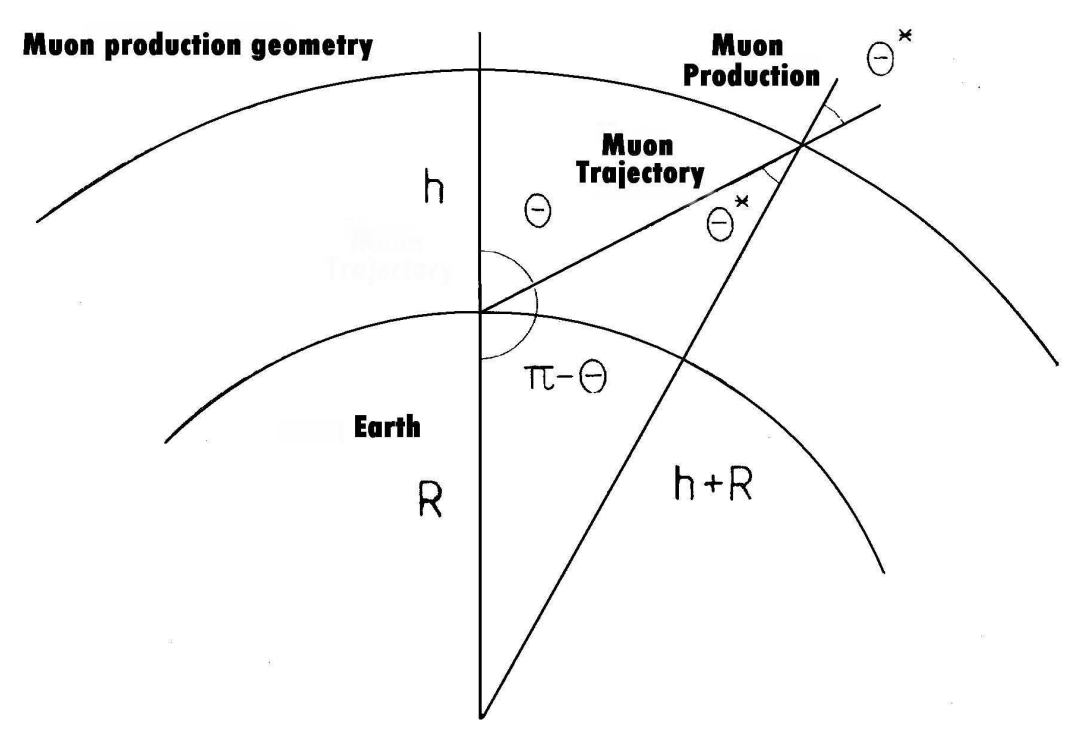
\includegraphics[width =0.6\textwidth]{figures/png/Screenshot_20240526_140716.png}
    \caption{The relation of the observed zenith angle of muons, $\theta^*$, to the zenith angle at the muon production point in the atmosphere, $\theta$. 
    $R$ is the radius of the Earth, Ref.\cite{guan2015parametrization}.}
    \label{fig:anglesinmuon}
\end{figure}

\subsection{Cosmics generation with CRY}
Among the Monte Carlo programs capable of simulating sea-level cosmic ray muons, 
CRY is the most widely used. CRY functions as a generator for air showers induced by primary cosmic rays. 
Its simulation relies on precomputed input tables derived from comprehensive MCNPX simulations of protons 
within the energy range of 1 GeV to 100 TeV, at the top of the atmosphere.

To produce muons along with their momentum and zenith angle distributions, 
the CRY package, developed by LANL, has been used. It uses data tables of primary 
cosmic rays with energies from 1 GeV to 100 TeV, generated using the Monte Carlo transport code MCNPX 2.5.0. 
The generation of muons and other secondary particles is governed by the pion and kaon decays. 
The package offers cosmic muon flux within a zenith angle range of 0-90°, following a cos$^2 \theta$ distribution, 
and energy ranges from 1-100 GeV, adhering to the Gaisser Tang parameterization. 
This package accounts for the dependence of cosmic-ray flux on various parameters, including altitude, latitude, and solar activity.
CRY provides muon flux data at three different altitudes: sea level, 2100 m, and 11300 m, with sea level being selected for the current study. 
The latitude is set at 41.8° N, corresponding to Fermilab. 
To avoid variations in primary cosmic-ray flux due to solar activity, a common day (6-21-2021) outside the maximum and minimum sunspot cycle has been chosen for the simulation.
While there are other packages designed to produce cosmic muons with specific energy and zenith angles, 
such as CORSIKA, CRY was chosen for this work due to its straightforward implementation and compatibility with Geant4.

\subsection{Simulation enviroment and coordinate system}\label{genplane}
In the Monte Carlo simulation, cosmic muons are uniformly generated within a horizontal plane approximately 11 m 
above the beam axis. The GEANT4 simulation also incorporates the effects of the external neutron shield surrounding the DS 
and the concrete ceiling of the Mu2e experimental hall. Starting from the generation plane, 
cosmic muons pass through the concrete ceiling and walls situated outside the experimental hall. 
As they propagate downwards to the detector, they interact with the materials within the building. 
The external neutron shield surrounding the DS consists of concrete ($\rho$=2.3 g/cm$^3$) and has a thickness of 
roughly 0.9 m, while the ceiling above the Mu2e experimental area comprises 1.8 m of concrete. 
The entire structure is enclosed within a volume of air at standard temperature and pressure.

The station was simulated in an extracted position, meaning it is placed outside the solenoid. 
Given that the Earth's magnetic field is approximately $4 \div 5 \times 10^{-5}$ T, 
and considering that the dimensions of the station are on the order of 1-2 m, 
along with the fact that the majority of particles under consideration have energies around $\sim$ 10 GeV, 
the curvature radius of the particles is approximately $R\sim p[\text{GeV}]/(B[\text{T}]\cdot 0.3) \sim 30$ m. 
This radius is significantly larger than the station's dimensions, allowing us to reconstruct particle trajectories as straight lines.
For this reason, the magnetic field of the Mu2e hall was turned off. 

Before starting explaining the event selection and the reconstruction, let me define the coordinate system, as shown in Figure \ref{fig:coordinate}.
\begin{figure}[!h]
    \centering
    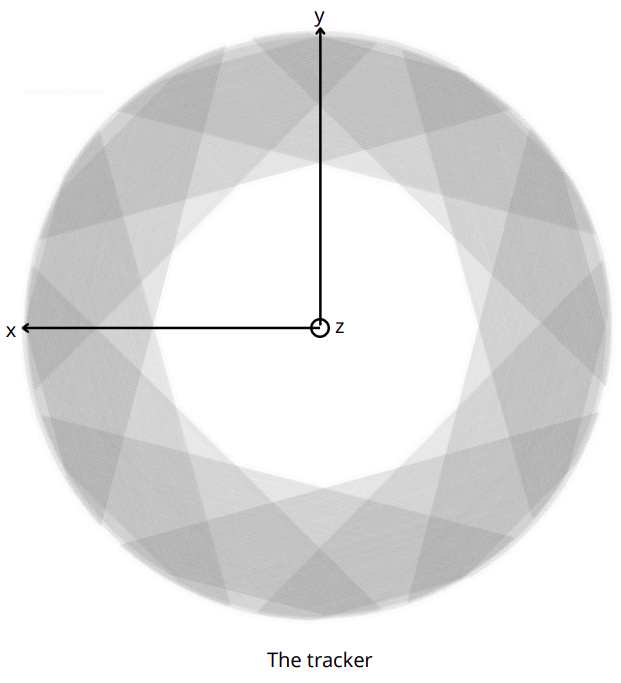
\includegraphics[width =0.5\textwidth]{figures/png/Screenshot_20240526_164527.png}
    \caption{Schematic view of a tracker station and definition of the coordinate used for the analysis.}
    \label{fig:coordinate}
\end{figure}
\section{Event selection}\label{eventselection}
Events in which a cosmic muon hits only the first station were chosen. 

Each straw can be parametrized as a straight line:
\begin{equation}\label{equaretta}
    (D_{x,i}t+M_{x,i},D_{y,i}t+M_{y,i},z_i)
\end{equation}
where $D_{x,i}$, $D_{y,i}$ are the straws' directions on $x$, $y$, while $M_{x,i}$, $M_{y,i}$ are the straws' midpoints on $x$, $y$. $z_i$ is the $z$ coordinate of the straw.
%One dimension is correlated with the other two, so we have just two informationful dimensions.
In this parametrization, the straws are all parallel on the $y-z$ plane.

Since two parallel straight lines (straws) define a three-dimensional plane of possible tracks, 
at least another pair of straws, uncorrelated with the initial two, is required to reconstruct a 
single straight line. The intersection of two planes forms a straight line. Therefore, at least four straws with different $z$ coordinates are necessary, 
so a number of hits per face greater than one was required.

Since more than one hit can occur in a single panel, another selection criterion was to choose events 
with fewer than three hit straws per panel. This criterion was chosen to minimize the error in position reconstruction.
\subsection{Panels illumination pattern}
To achieve accurate timing calibration, it is essential to have uniform illumination of the hits across each panel. 
Using only the conditions outlined in Section \ref{eventselection}, the Monte Carlo hits were plotted in the reference frame of the panel. 
The result is shown in Figure \ref{fig:illumination} for panel 0 of plane 0, which corresponds to the upper right panel in Figure 
\ref{fig:coordinate}. 
\begin{figure}[!h]
    \centering
    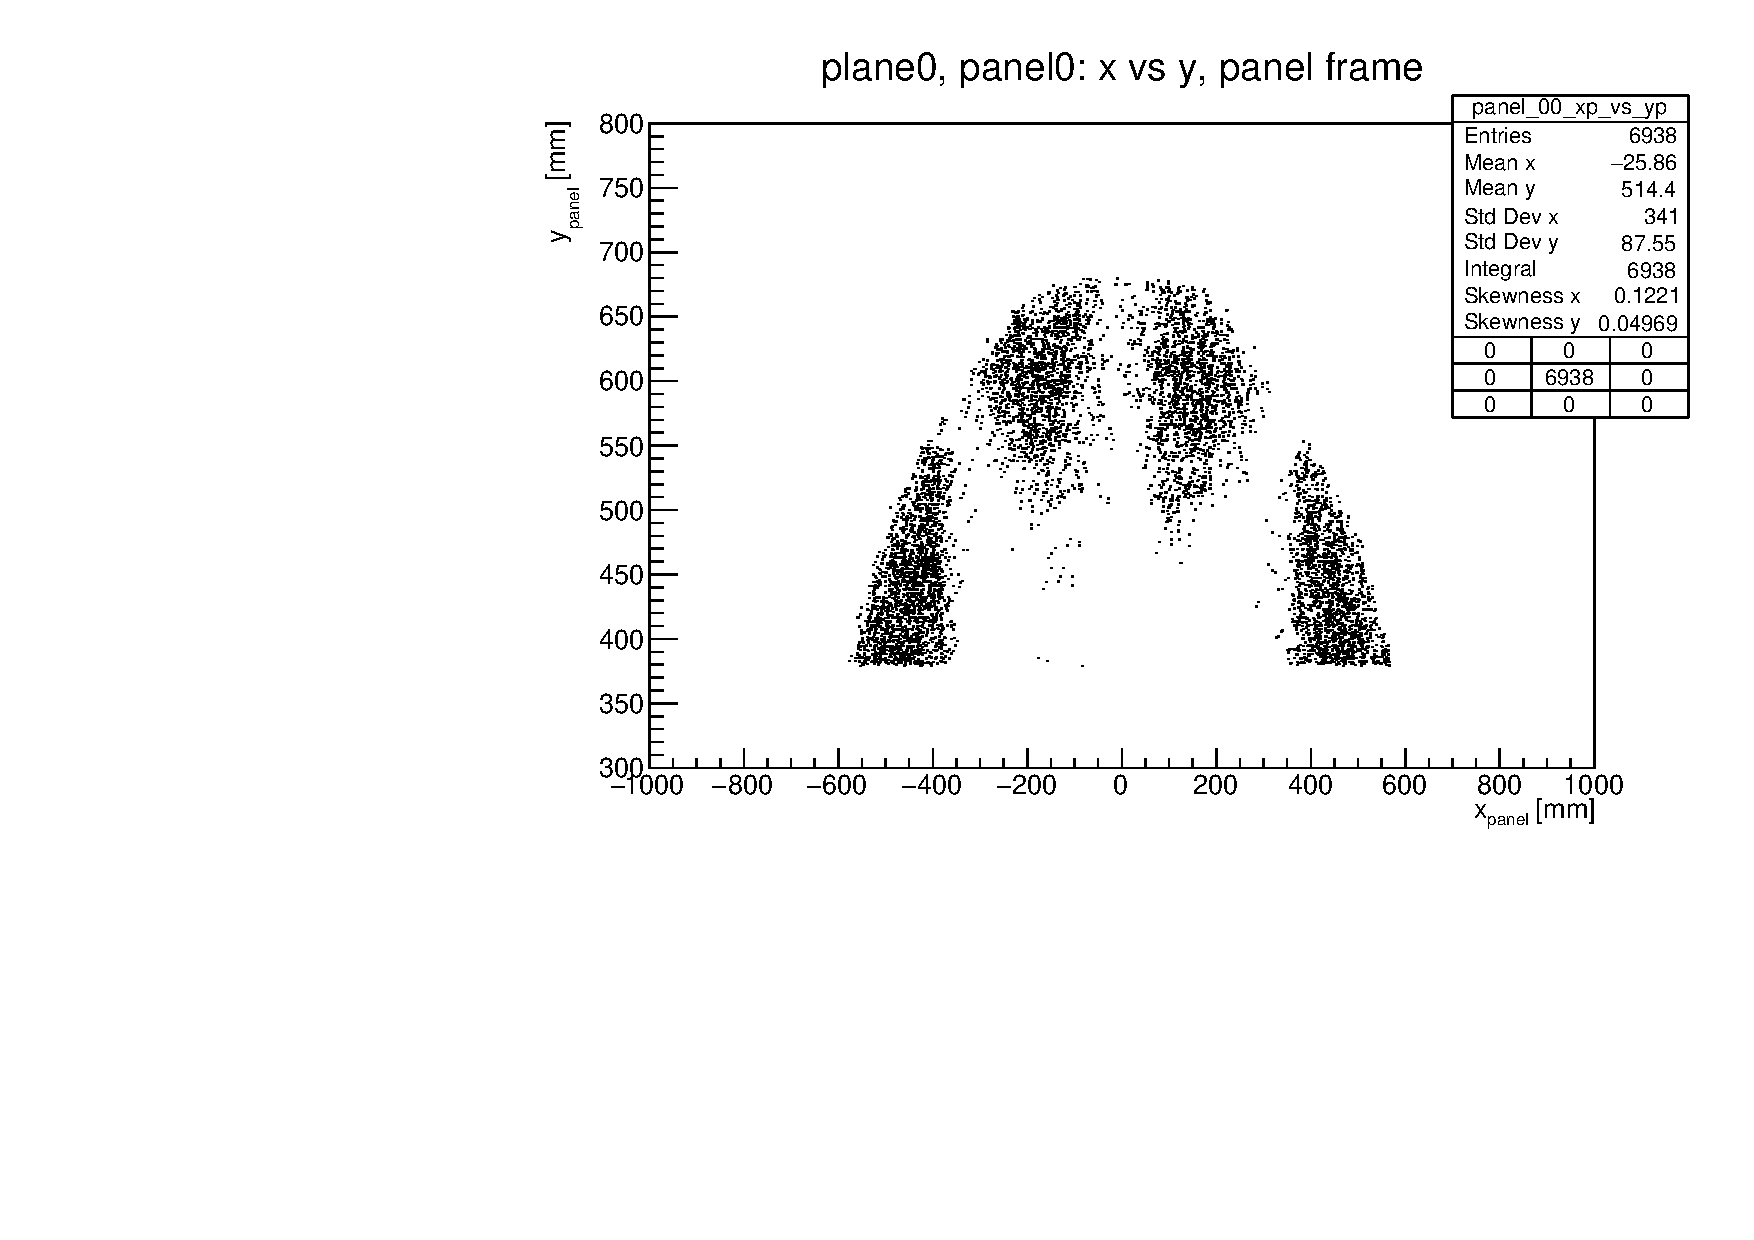
\includegraphics[width =0.8\textwidth]{figures/pdf/xp_vs_yp_panel0.pdf}
    \caption{Illumination of Monte Carlo hits on panel 0, plane 0, selecting cosmics that traverse at 
    least four panels across four distinct faces of the station, with fewer than three hits per panel.}
    \label{fig:illumination}
\end{figure}
Similar patterns were observed for all panels in both planes, as shown in Appendix \ref{appendix2}. 

The illumination is spotty and non-uniform. This unusual illumination is due to the panels' overlap areas being located at their extreme edges, as shown in Figure \ref{fig:coordinate}. 
The overlaps select specific cosmic directions in the $y$-$z$ plane. 
To better visualize the selected directions, the Monte Carlo $m_{yz}=\Delta y /\Delta z$ distribution has been plotted in Figure \ref{fig:myz}.
There are no tracks corresponding to the $m_{yz}\sim 0$, which are horizontal tracks, as one could expect. The vertical tracks, 
which correspond to $m_{yz} \rightarrow \infty$, are also not selected by our algorithm, since no panels would be hit in these conditions. Since most of the cosmics' tracks are vertical, 
this results in a very low rate too, that will be investigated better in Section \ref{ratetracker}. The most selected directions are those with $|m_{yz}| \sim 1$, which represent cosmics with 
an angle of approximately 45°.
\begin{figure}[!h]
    \centering
    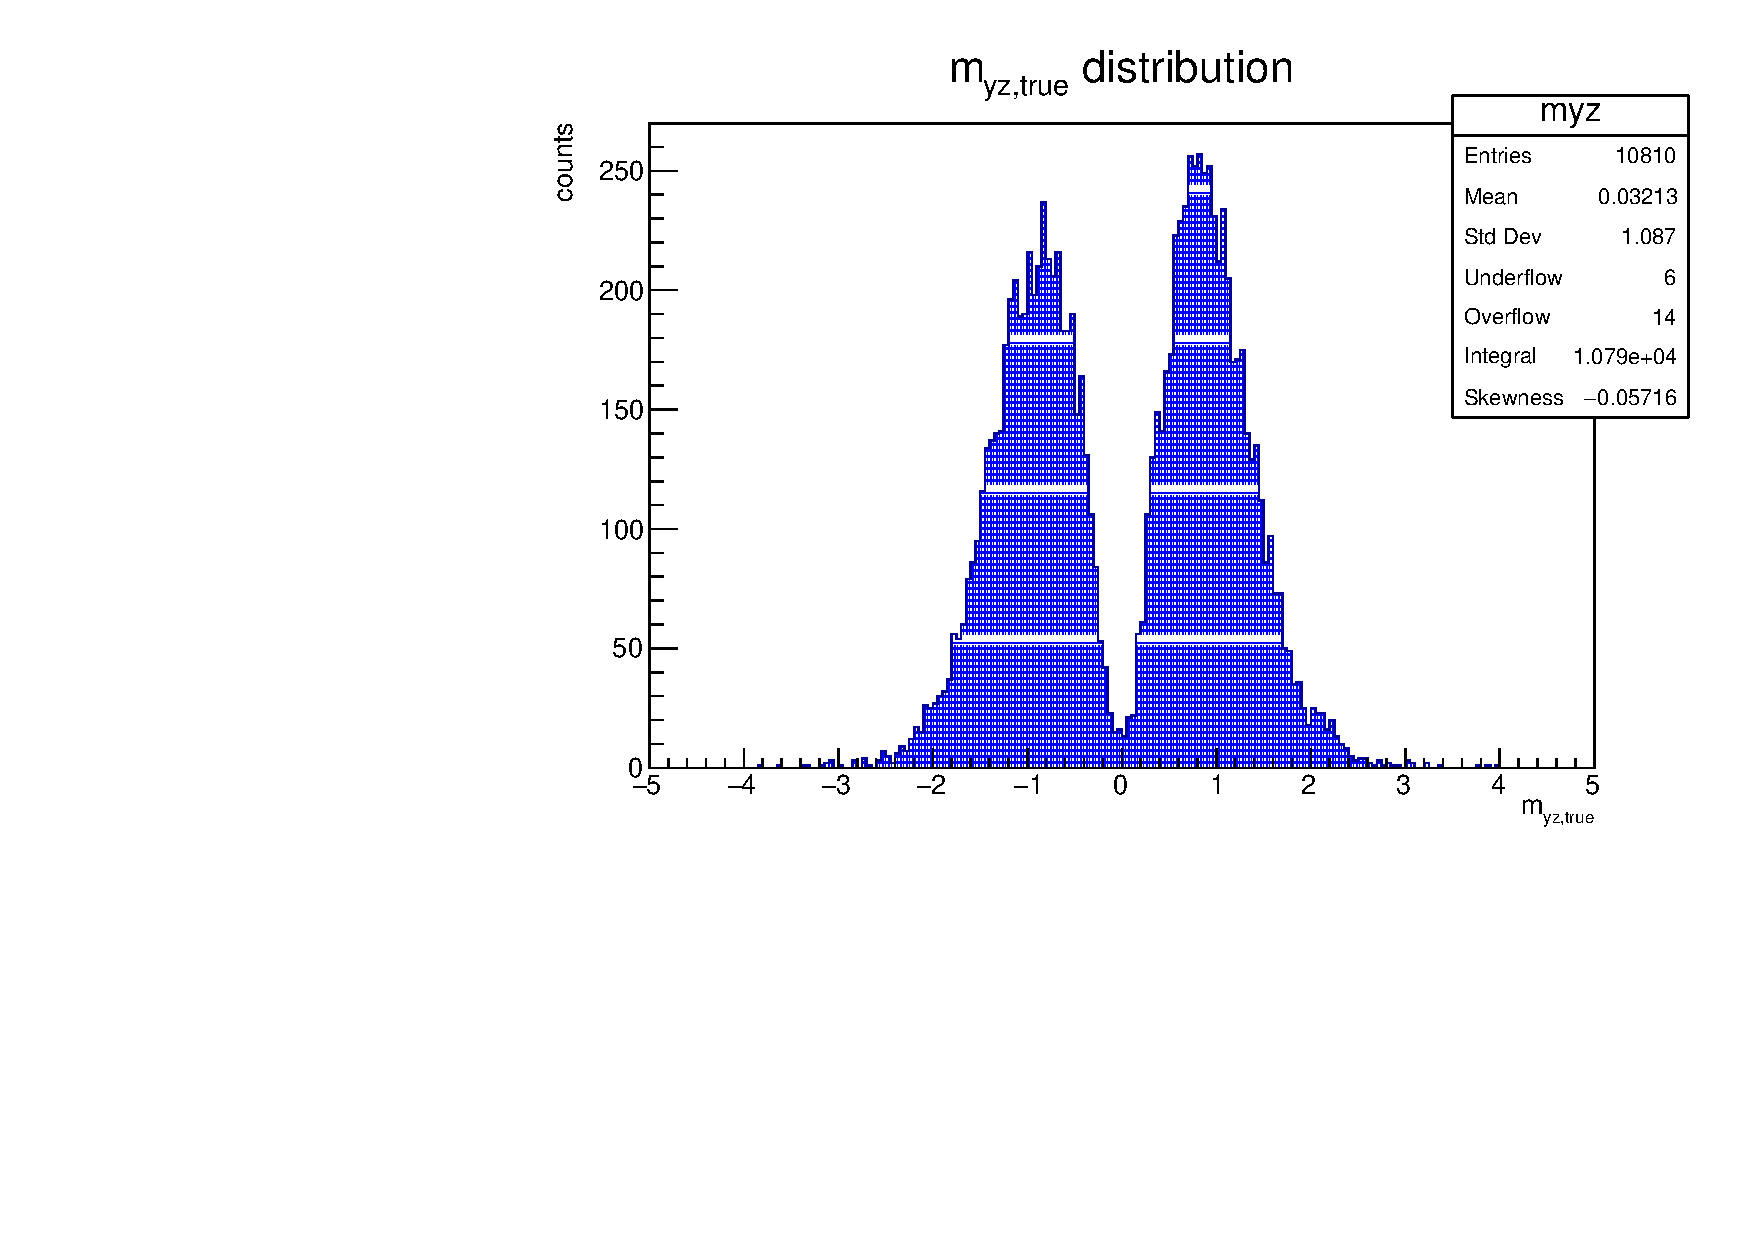
\includegraphics[width =0.8\textwidth]{figures/pdf/myz.pdf}
    \caption{The Monte Carlo $y-z$ direction distribution of cosmic rays ($m_{yz}=\Delta y /\Delta z$).}
    \label{fig:myz}
\end{figure}

Additionally, Figure \ref{fig:illumination} shows that there are almost no hits in the panel central region, which could result in waveform non-linearities.
Specifically, if particles pass near the end of the straw, signals are wider, and wider signals have greater charge and 
height compared to others. Consequently, the leading edge would be very sharp, potentially causing timing systematics.

\subsection{Rate}\label{ratetracker}
The rate of generated events, on the horizontal plane above the beam axis, is computed by integrating the flux on the solid angle, on the muon energy described in Section \ref{genplane}:
\begin{equation}
   R= \int \frac{\text{d} I}{d E_\mu \text{d} \Omega \text{d} t \text{d} S} \text{d} S_{\perp} \text{d} \Omega \text{d} E_\mu
    \end{equation}
where $\text{d}S_\perp= \text{d}S \text{cos}\theta$ is the projection of the surface element on the plane perpendicular to the cosmics flux. 
The energy and angle ranges selected for this simulation are 0.5 GeV < $E_\mu$ < 500 GeV, representing the 
muons that are not absorbed in the concrete located above the tracker, and 0° < $\theta^*$ < 90°. 
Considering a generation plane of $\sim 5$ m$^2$, the result is $R \sim 380$ Hz. 
%The rate of cosmic muons detected by each straw, $R_{straw}$, can be easily obtained as:
%\begin{equation}
%    R_{straw}=\frac{R}{(N_{faces}\cdot N_{panels}\cdot N_{straws} )}
%\end{equation}
%where $N_{faces}=4$ is the number of hit faces, $N_{panels}=3$ is the number of panels in one face and $N_{straws}=96$ is the number of straws in one panel.
%The resulting rate is about 0.5 Hz. This simple computation does not take into account the complicated tracker geometry and the station orientation.
%Let us normalize by a factor that is the ratio between the number of selected events and the total number of produced events, which is about 
%$\sim10^{-3}$. The rate then changes to $\sim$ mHz. 
%To perform a proper calibration, at least $\sim$1000 hits per straw are needed, which requires at least 8 days of data taking.
%This rate calculation is quite straightforward, but the duration required for such a simple calibration is notably long.
In the simulation, 2$\times 10^8$ cosmic muons\footnote{The number of selected events was chosen to be 2$\times 10^8$, since the number of cosmics that 
hit a station is about 8$\times 10^5$ and this is a good number of events to perform a reasonable calibration.} were generated on the horizontal plane. 
From this number, it is possible to compute the time required for calibration, that is
$\Delta t = N_{gen}/R\sim 6$ days. 
This rate calculation is straightforward, but the time needed for such a simple calibration is excessively long.
\section{Reconstruction of a straight cosmic track}
The only information about a straw are, as mentioned in equation \ref{equaretta}:
\begin{itemize}
    \item the straw direction $(D_{x,i},D_{y,i})$;
    \item the straw midpoints $(M_{x,i},M_{y,i})$;
    \item the straw $z_i$ coordinate.
\end{itemize} 
The reconstruction process starts with hit reconstruction. The digital
signals coming from the tracker are converted to physical time and position making an object
called $StrawHit$. To improve the hit spatial resolution adjacent $StrawHit$s in a panel, which are
due to the same particle, are combined to form the object called $ComboHit$.
This object effectively represents a straw with its direction aligned to the straw directions and its midpoint 
being the average of the hit straw midpoints in that panel. Since four panels in four different faces have been selected,  
four $ComboHit$s are reconstructed within a station. The new $ComboHit$ midpoints will be referred to as $(x_{m,i}, y_{m,i}, z_{m,i})$.
Two $ComboHit$s from different faces within the same plane are combined to form a $StereoHit$. 
The $x$ and $y$ coordinates of the $StereoHit$ are determined by the intersection point of the two 
$ComboHit$s. The $z$ coordinate of the $StereoHit$ is the average of the $z$ coordinates of the $ComboHit$s.
The situation is reproduced in Figure \ref{fig:stco}.
\begin{figure}[!h]
    \centering
    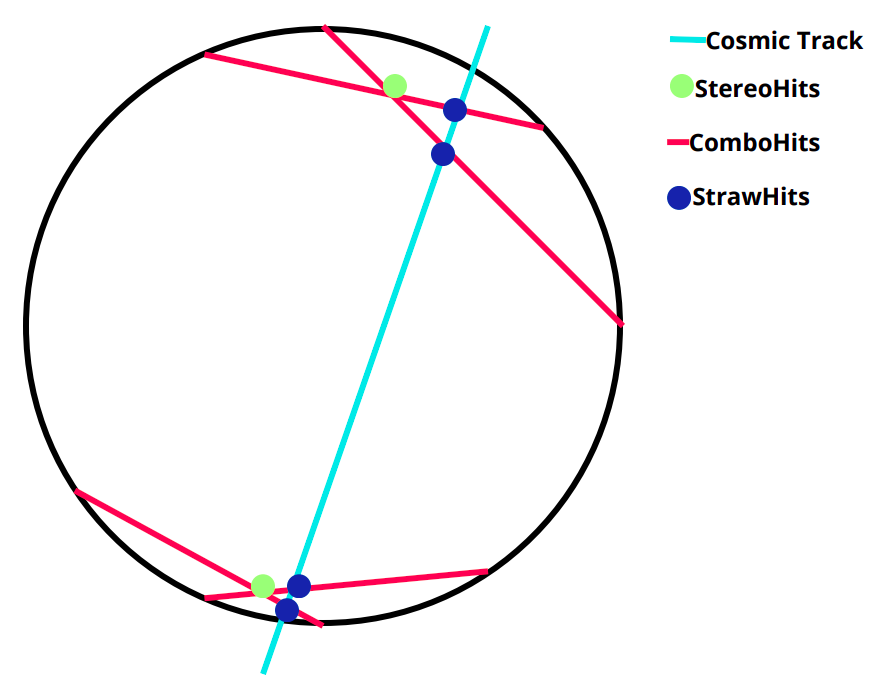
\includegraphics[width =0.6\textwidth]{figures/png/Screenshot_20240601_195651.png}
    \caption{Schematic view of a cosmic muon (light blue) hitting the vertical oriented station. The red lines are the $ComboHit$s, the dark blue dots 
    are the $StrawHit$s and the green dots are the $StereoHit$s.}
    \label{fig:stco}
\end{figure}
Considering only one plane and the following equations as the $x-y$ $Combo Hit$s equations:
\begin{equation}
    \begin{aligned}
        y&=\frac{v_1}{u_1}(x-x_{m,1})+y_{m,1} \\
        y&=\frac{v_2}{u_2}(x-x_{m,2})+y_{m,2} 
    \end{aligned}
    \end{equation}
where $u_i$ is the $ComboHit$ $x$ direction and $v_i$ is the $ComboHit$ $y$ direction, the $StereoHit$ coordinates will be:
\begin{equation}\label{x}
    \begin{aligned}
x&=\frac{u_1 u_2(y_{m,1}-y_{m,2}+\frac{v_2}{u_2}x_{m,2}-\frac{v_1}{u_1}x_{m,1})}{v_2 u_1 - v_1 u_2}\\
y&=\frac{v_2}{u_2}\left(\frac{u_1 u_2(y_{m,1}-y_{m,2}+\frac{v_2}{u_2}x_{m,2}-\frac{v_1}{u_1}x_{m,1})}{v_2 u_1 - v_1 u_2}-x_{m,2}\right)+y_{m,2}
\end{aligned}
\end{equation}
In two different planes, there are two $StereoHit$s available, allowing for the reconstruction of the track on $x-y$ and $y-z$ planes. 
Referring to these $StereoHit$s as $(x_1,y_1,z_1)$ and $(x_2,y_2,z_2)$ respectively, the final track slope on $x-y$ plane will be 
denoted as $m_{xy}$, while on the $y-z$ plane it will be denoted as $m_{yz}$. The corresponding $y$-intercepts will be $q_{xy}$ and $q_{yz}$.
The formulas for computing these parameters are as follows:
\begin{equation}
    \begin{aligned}
m_{xy}&=\frac{y_2-y_1}{x_2-x_1}\\
q_{xy}&=-m_{xy} \cdot x_1+y_1
\end{aligned}
\end{equation}
\begin{equation}
    \begin{aligned}
m_{yz}&=\frac{y_2-y_1}{z_2-z_1}\\
q_{yz}&=-m_{yz} \cdot z_1+y_1
\end{aligned}
\end{equation}
To determine the four hit positions of the reconstructed track on the panels, we need to intersect the track with the panels' $z_i$ coordinates. 
The reconstructed hits on the panels will be denoted as $R_{x,i}$ and $R_{y,i}$.
\begin{equation}
    \begin{aligned}
 R_{y,i}&=m_{yz}\cdot z_i+q_{yz}\\
 R_{x,i}&=\frac{(m_{yz}\cdot z_i+q_{yz}-q_{xy})}{m_{xy}}
\end{aligned}
\end{equation}
The bias on the longitudinal position is the difference between the reconstructed coordinate and the true Monte Carlo position in the panel frame.

\section{Results}

Our target is to achieve a longitudinal resolution better than 4 cm, thus ensuring that every bias on the reconstructed coordinate 
remains below this threshold. For each panel, I plotted the reconstructed longitudinal coordinate, as shown for panel 0 in Figure \ref{fig:recx}. 
Similar patterns were observed for all panels. In this distribution, the bumps are a consequence of the four-hit face requirement and the panels' overlap areas being located at the extreme edges. 
It is important to observe is that different bumps correspond to different straws, as can also be seen in Figure \ref{fig:illumination}.
\begin{figure}[!h]
    \centering
    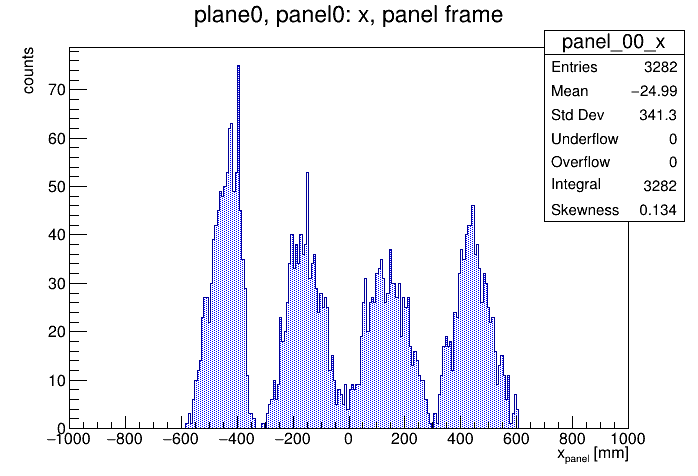
\includegraphics[width=0.8\textwidth]{figures/png/x_panel0.png}
    \caption{The reconstructed longitudinal coordinate in the 0th panel frame.}
    \label{fig:recx}
\end{figure}
The positional bias between the reconstructed and true longitudinal coordinates is plotted in 
Figure \ref{fig:bias}. The true coordinate is the mean coordinate of the Monte Carlo hits. The bias range is approximately [-6, 6] cm, 
indicating a significant systematic factor affecting the reconstructed hit. The distribution is nearly symmetric, similar for all panels. 
There are four peaks corresponding to the four different spots shown in Figure \ref{fig:illumination}.

\begin{figure}[!h]
    \centering
    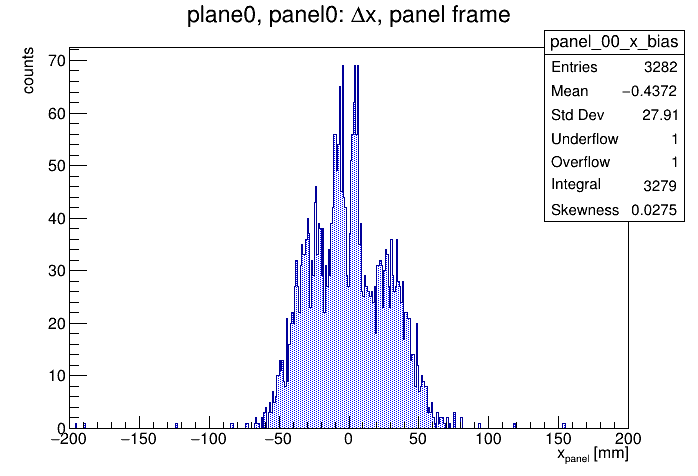
\includegraphics[width=0.8\textwidth]{figures/png/panel_00_x_bias.png}
    \caption{The difference between the reconstructed and the true longitudinal coordinate in the 0th panel frame. 
    The true coordinate is the mean coordinates of Monte Carlo hits.}
    \label{fig:bias}
\end{figure}
The 2D distribution of the longitudinal bias versus the true position, shown in 
Figure \ref{fig:rec2D}, shows four different spots on the $x$ axis corresponding to 
the overlap regions. Each spot refers to different straws. The two spots on the $y$ axis correspond to cosmics with different orientations. 
The first spot (CAL side) correspond to 90° panels overlap.
\begin{figure}[!h]
    \centering
    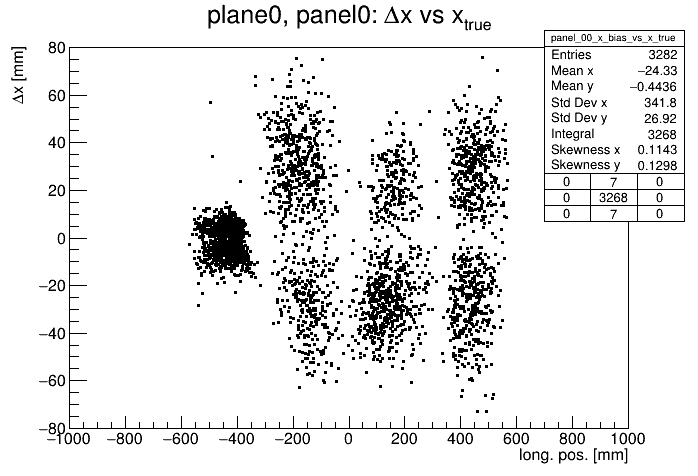
\includegraphics[width=0.8\textwidth]{figures/png/panel_00_x_bias_vs_x.png}
    \caption{The 2D histogram of the longitudinal bias versus the true longitudinal coordinate.}
    \label{fig:rec2D}
\end{figure}
To assess the systematic impact on the reconstructed coordinates, it is essential to visualize the TProfile of the bias versus the true coordinates. 
Profile histograms are used to represent the mean value of $y$ and its error for each bin in $x$. 
The default displayed error is the standard error on the mean. 
The profile is depicted in Figure \ref{fig:profile}. It reveals a systematic effect in determining the 
longitudinal position within a range exceeding [-4,4] cm. The initial portion of the histogram (CAL side) 
corresponds to the overlap of 90° panels. This plot indicates that the mean may not serve as an accurate estimator of the bias. 
Under these conditions, the calibration is expected to become challenging.
\begin{figure}[!h]
    \centering
    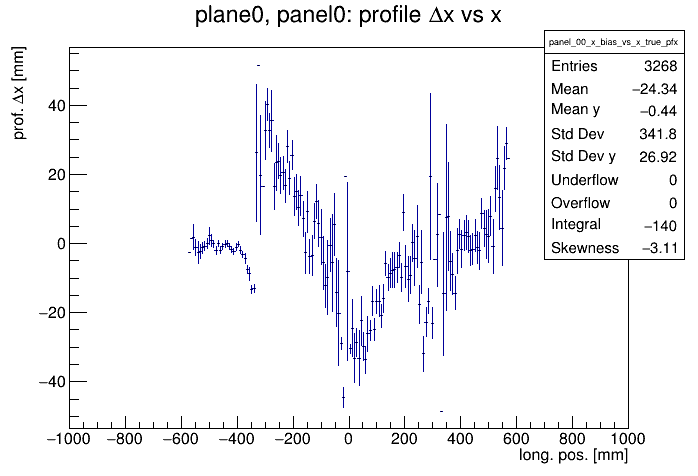
\includegraphics[width=0.8\textwidth]{figures/png/panel_00_x_bias_vs_x_prof.png}
    \caption{The profile of the longitudinal bias versus the true longitudinal coordinate.}
    \label{fig:profile}
\end{figure}
The main issue with this type of reconstruction lies in the fact that $m_{yz}=\frac{\Delta y}{\Delta z}$ 
is not accurately reconstructed. Consequently, the reconstructed coordinates depend on this value, as demonstrated in \ref{}. 
This discrepancy arises when the true hit position, far from the midpoint of the straws, results in incorrectly reconstructed tracks'
direction on the $y-z$ plane, leading to horizontal cosmic rays being reconstructed. 
Figure \ref{fig:myzrec} shows the reconstructed $m_{yz}$ distribution, highlighting a significant peak at the value of 0, 
indicating horizontal cosmic rays, which are not possible in reality. This plot needs to be compared with the true $m_{yz}$ distribution, Figure \ref{fig:myz}.


\begin{figure}[!h]
    \centering
    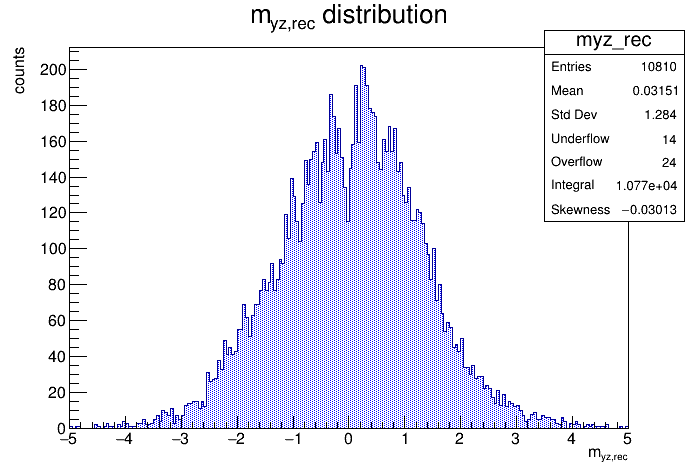
\includegraphics[width=0.8\textwidth]{figures/png/myz_rec.png}
    \caption{The reconstructed $y-z$ direction distribution of cosmic rays ($m_{yz}=\Delta y /\Delta z$).}
    \label{fig:myzrec}
\end{figure}
\section{Conclusions}
This chapter demonstrated that the vertical orientation for calibrating a station is not optimal. This is due to several reasons:
\begin{itemize}
    \item The selection criteria in Section \ref{eventselection} select cosmic muons with orientations that affect panel illumination. 
    The illumination is non-uniform, and moreover, there are almost no hits in the central region of the panel, which could result in waveform non-linearities;
    \item The rate of cosmic events is $R \sim 380$ Hz, and the expected duration of the calibration is about 6 days without interruptions, 
    which is excessive for the simple calibration we intend to perform;
    \item The bias range is approximately [-6, 6] cm. The 2D distribution of the longitudinal bias versus the true position shows 
    four distinct spots on the $x$ axis corresponding to the overlap regions. Each spot refers to different straws.
\end{itemize}
Therefore, an alternative orientation or method should be considered to optimize the calibration process and achieve more accurate results.

%yongi cap 3.1.5.2
%con il tracker in orizzontale , dato che le tracks sono verticali colpirebbero per panel sicuro almeno 2 straws che sono sovrappposte e quindi in totale 8, se hanno una certa angolazione anche 12






%yongi:
%As discussed in Chapter 3, the Mu2e Tracker panels need to satisfy a series of performance
%requirements for successful operations and the designed resolution. While various individual
%component and single panel tests in the past confirmed their respective effectiveness, it was of great
%interest to extend the tests to a system of multiple panels over a longer period of time under a more
%realistic setup (i.e., similar to that of the actual experiment setup), and to get better quantitative
%understandings of the detector performances. Hence, a VST was conducted.
%The overall goal of the VST was to “exercise the full tracker operation and readout chain,
%from the amplified wire signal to its storage in digitized format” [1]. The test used a whole plane of
%six panels from panel pre-production,1 which was 1/36 of the full Tracker.
%The VST contained two phases. In the first phase, the plane was laid horizontally on a
%test bench for diagnostics and horizontal position runs, as shown in Figure 5.1(a). In the figure
%the supporting systems, including gas lines, DC-to-DC converters for low voltage supplies, high
%voltage supplies, and the Raspberry Pi (marked as RPi) for panel controls, are all labeled.2 In this
%phase, the plane operations and performances were checked. The plane data output to the DAQ
%server through the optical fiber links (see Chapter 4 and Appendix B) were finalized and tested.
%Small cosmic-ray datasets werereconstruction of the track longitudinal position taken to verify the ability to synchronize data taking among the
%panels. And 55 Fe source scan studies were performed for calibrations. The second phase of the



%reconstruction of the track longitudinal position
%tracker/vstplan
%We also plan to take significant amounts of cosmic ray data in at least two configurations. First, cosmic ray data will be taken with the plane in the current horizontal
%position. This will be taken using a modified readout scheme involving the serial
%connection as described above. Software exists to take the output raw data and manually convert it into an art format that can be processed by the official Mu2e software
%packages. This first cosmic data will be used to confirm the functionality of the system - including a cross-check of the panel to panel time synchronization, and the
%overall timing measurement performance. 
%Additionally, enough statistics could allow
%for important preliminary calibrations of delta-t resolution, longitudinal propagation
%velocities, efficiencies, and channel to channel variations. The fairly uniform distribution and wide phase-space of tracks in the horizontal configuration can make these
%analyses more straightforward than in the vertical configuration. Additionally a better measure of the expected showering will allow an improved analysis of vertical data.
%Finally, it may be possible to make some measure of the difference between vertical
%and horizontal straw alignment compared to expectations from Duke measurements
%and gravitational sag
%Later, the plane will be positioned vertically and another month of cosmic data
%will be taken. At this point readout may be through the fiber and DTC for improved
%livetime. As described above we will move towards automatic processing of this
%data and have it copied and backed up to tape. This data will be most useful for
%testing the track reconstruction. There exists software for reconstructing cosmic
%tracks without a magnetic field, and it has been tested in a limited fashion with
%data from a single vertical panel (docdb-33914). The implementation for a single
%plane in either horizontal or vertical configuration is being developed.
%Finally, a more thorough calibration of the plane can be done using a systematic
%scan across each panel with an Fe55 source. This will allow further measurements of
%the response as a function of straw and position, and a determination of the variability
%between panels.